% Preview source code

%% LyX 2.0.6 created this file.  For more info, see http://www.lyx.org/.
%% Do not edit unless you really know what you are doing.
\documentclass[english]{article}
\usepackage[T1]{fontenc}
\usepackage[latin9]{inputenc}
\usepackage{float}
\usepackage{amstext}
\usepackage{graphicx}

\makeatletter

%%%%%%%%%%%%%%%%%%%%%%%%%%%%%% LyX specific LaTeX commands.
\newcommand{\lyxmathsym}[1]{\ifmmode\begingroup\def\b@ld{bold}
  \text{\ifx\math@version\b@ld\bfseries\fi#1}\endgroup\else#1\fi}


\makeatother

\usepackage[english]{babel}
\begin{document}

\title{A Pedestrian Simulation }


\author{Daniel Parisi, Agustin Marseillan, Castiglione Gonzalo}
\maketitle
\begin{abstract}
En este paper se presenta un nuevo método para simular peatones virtuales
basado en el modelo de la fuerza social. En el modelo presentado,
cada peatón posee un punto movil frente a el y camina siempre hasta
este. Este punto representa un objetivo a corto plazo que se debe
cumplir. Cada peatón se encarga de mover este punto según a donde
necesite llegar. 
\end{abstract}
keywords:

pedestrian, collision avoidance, future, force model

\pagebreak{}


\section{Introduccion}

// Daniel tiene ya preparada una introducción\\


El transito de personas es un factor de suma importancia en el análisis
y diseño de instalaciones tales como edificios públicos, peatonales,
estaciones de trenes, entre otros. 

// Hace mucho tiempo que se viene estudiando a las personas en grupo
y se sabe que 

// Existen efectos de comportamiento colectivos de auto organización
tales como cuellos de botellas, formaciones en filas, bloqueos. 

// Decir porque una simulación de peatones es útil para estas situaciones.\\


Analizar estructuras de transito de peatones usando los cambios propuestos
para el modelo de la fuerza social. Implementar una interfaz gráfica
para poder visualizar los resultados de cambiar el modelo y cada uno
de los parámetros


\section{Modelo de agentes}

El actual modelo se encuentra definido uncamente por peatones. Estos
se encuentran definidos por: 
\begin{itemize}
\item Area circular 


Representa el área física que ocupa el peatón. El radio del círculo
es generado aleatoriamente con el fin de representar peatones diferentes.
El rango de valores se distribuye uniformemente en el intervalo $[0.25,0.29]$
$[cm]$.

\item Objetivo a largo plazo 


Se represa por por un segmento de recta, al tocarse, se considera
que el objetivo fue cumplido. Se permite la definición de múltiples
objetivos, en cuyo caso, se deben cumplir todos de manera secuencial
según el orden en que fueron especificados.

\item Posición objetivo a corto plazo 


Llamado Future, representa un punto a corta distancia del peatón,
que debe ser alcanzado. El seguir este punto garantiza que se va a
cumplir el objetivo a largo plazo, aunque podría recorrerse un camino
no óptimo en cuanto a distancia recorrida. Este punto es un punto
móvil y se puede aplicar fuerzas sobre el. La masa de este punto fue
definida fija con un valor de $1$ $[kg]$.

\item Velocidad objetivo 


Con el fin de representar peatones que puedan estar apurados o tranquilos,
se definió la velocidad máxima deseada de un peatón de manera aleatoria.
El rango de valores se encuentra definido en el intervalo $[1,1.6]$
$[m/s]$.

\item Distancia de reacción 


Representa la distancia a la cual va a tratar de posicionar de sí
mismo un peatón su propio future. Una mayor distancia representa un
peatón que reacciona más rápido a una posible colisión.

\end{itemize}
En la siguiente imagen se puede observar de manera gráfica la descripción
de un peatón:

\begin{figure}[H]
\begin{centering}
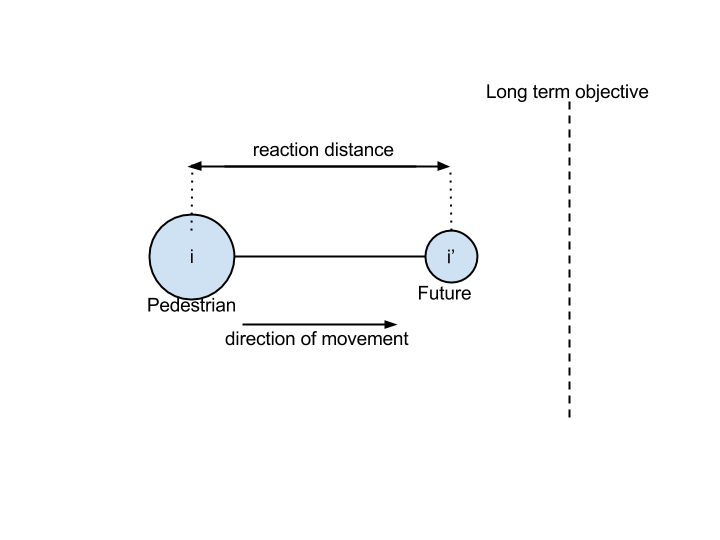
\includegraphics[scale=0.5]{pedestrian-top}\caption{Vista superior de un peaton}

\par\end{centering}

\end{figure}


// FALTA ESPECIFICAR: 

// i representa un peaton e i\textquoteright{} representa el future
del peaton 

// que se usa Euler para el calculo del dx de cada cuerpo 

// el dt usado


\section{Funcionamiento}

Cada peatón en la simulación posee un objetivo a largo plazo que sea
desea que alcance. Para asegurar que esto se cumpla, se trata siempre
de mantener su future (objetivo a corto plazo) alineado con el camino
más óptimo hacia su objetivo. Sin embargo, pueden darse casos en donde
exista uno o más peatones en el camino, obligando a tener que buscar
rutas alternativas. Es en estas circunstancias en donde el objetivo
a corto plazo va a cambiar su dirección según corresponda. 

El movimiento de los peatones se realiza de manera sincrónica y se
calcula en cuatro etapas: 
\begin{enumerate}
\item Cálculo de la fuerza sobre sobre cada future. 
\item Actualización de la posición de cada future. 
\item Cálculo de la fuerza sobre cada peatón. 
\item Actualización de la posicion de cada peatón. \\

\end{enumerate}
En donde, cada etapa se define de la siguiente manera:
\begin{enumerate}
\item Cálculo de la fuerza sobre sobre cada future. 


En esta etapa, lo que se va a hacer es calcular la fuerza que sufre
cada uno de los futures existentes debido a la existencia de otros
peatones. Esta se realiza sólo cuando la distancia entre el peatón
y su future se encuentra por encima de cierto valor. Esto es así ya
que a altos niveles de densidad de personas. Uno ya no intenta moverse
ya que simplemente es arrastrado por la masa de gente. \textbf{(verificar
si es correcta esta última frase)}


En el caso contrario, cuando que un peatón se encuentra habilitado
para moverse, se realiza un filtro de todos aquellos peatones que
se encuentran a sus espaldas, ya que estos no son casos que afectam
la trayectoria de la persona. La condición que debe cumplirse para
considerar un peatón $j$ como detrás del peatón $i$ es: 


\[
v=normal(i,center.target.i)
\]
\[
v_{x1x0}=v_{x1}-v_{x0}
\]
\[
v_{x1x0}.x*(i.y-v_{x0}.y)-v_{x1x0}.y*(i.x-v_{x0}.x)>0
\]



Una vez filtrado los peatones, simplemente se calcula por cada future
restante, la fuerza de repulsión entre estos. Este se realiza utilizando
la fórmula: 


\[
F_{i',j'}=\alpha e^{-dist(i',j')/\beta}
\]



en donde $\alpha$ y $\beta$ son constantes predefinidas y fijas.
Los valores que se usaron son $?$ y $?$ respectivamente. Esto produce
que los peatones tienda siempre a alejarse de grandes multitudes más
de lo que aleja de una sola persona. Si la suma de todas las fuerzas
ejercidas sobre todos los demás futures $j\lyxmathsym{\textquoteright}$
al future $i\lyxmathsym{\textquoteright}$ es menor que cierto umbral,
entonces se desprecia esta fuerza y el future $i\lyxmathsym{\textquoteright}$
simplemente es posicionado sobre la recta que une al peatón $i$ con
su objetivo a largo plazo a distancia que indique la distancia de
reacción del peatón. 


\begin{figure}[H]
\centering{}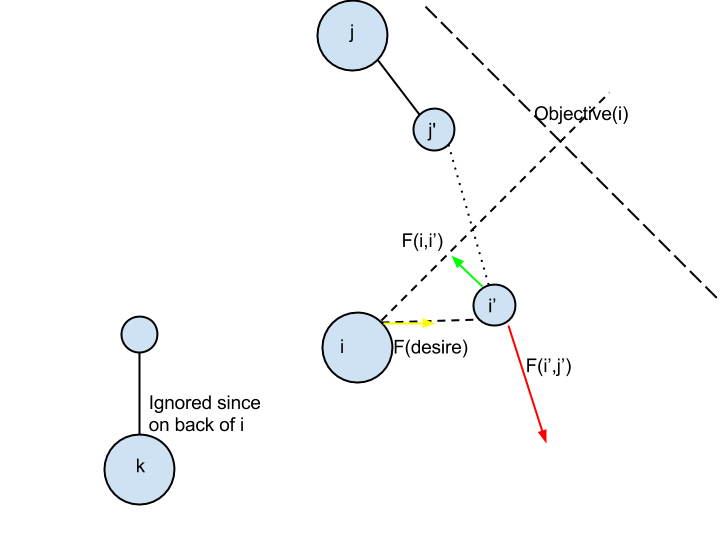
\includegraphics[scale=0.5]{pedestrian-top-forces}\caption{Fuerzas que actúan sobre el Future $i'$}
\end{figure}


\item Actualización de la posición de cada future. 


En esta etapa, simplemente se actualiza la posición de cada future
según el cálculo de la fuerza aplicada en la etapa previa. Este cálculo
se realiza utilizando las fórmulas Eulerianas.

\item Cálculo de la fuerza sobre cada peatón. 


El peatón siempre se mueve hacia la dirección en la que apunta su
future y de acuerdo a la fuerza de deseo.


Esta fuerza representa la atracción que un peatón $i$ ejerce sobre
sí mismo a fin de dar un paso hacia su future y tratar de alcanzarlo.
Esta definida por la siguiente fórmula: 


\[
F_{deseo}=\frac{dist(i',i)}{dist_{react}}\frac{v_{desire}-v_{curr}}{\tau}\frac{i'-i}{|i'-i|}
\]



En donde $\tau=0.5$

\item Actualización de la posición de cada peatón. 


La nueva posicion de cada peatón es calculada en esta etapa utilizando
las mismas fórmulas mencionada en la etapa 2.

\item Validación del modelo 


\textbf{// Poner Graficos indicando distancias y esquemas del future
y la particula. }

\item Conclusiones


\textbf{// agregar al final futuras opciones que se abren con este
trabajo}

\end{enumerate}
\pagebreak{}
\begin{enumerate}
\item Referencias


{[}1{]}... Karamouzas?


{[}2{]}...\end{enumerate}

\end{document}

